\documentclass[10pt,a4paper,nofonts]{ctexart}
\usepackage[utf8]{inputenc}
\usepackage{xeCJKfntef}
\def\tjf{{\tt{田劲锋}}}
\def\titlec{大学物理}
\usepackage[b5paper,margin=2cm]{geometry} % 页面设置
\usepackage[unicode,breaklinks=true,
colorlinks=true,linkcolor=black,anchorcolor=black,citecolor=black,urlcolor=black,
pdftitle={\titlec},pdfauthor={\tjf}]{hyperref}
\usepackage{latexsym,amsmath,amssymb,bm}
\usepackage[inline]{enumitem} % 调整列表样式
\usepackage{multicol} % 分栏
\usepackage{color,xcolor}
\usepackage{tikz}
\usepackage{wrapfig}

% \setmainfont{Times New Roman}
\setCJKmainfont[BoldFont={SimHei}]{SimSun}  % 主要字体: 宋体、黑体
\setCJKsansfont[BoldFont={STZhongsong}]{STFangsong} % 次要字体: 仿宋、中宋
\setCJKmonofont{KFKai} % 等宽字体: 楷体

\CJKsetecglue{\hspace{0.1em}}
\renewcommand\CJKglue{\hskip -0.3pt plus 0.08\baselineskip}
\frenchspacing
\widowpenalty=10000
\linespread{1.2} % 行距

\pagestyle{plain}

\setlist{noitemsep}
\setlist[itemize]{topsep=0pt,partopsep=0pt,itemsep=0pt,parsep=0pt,labelindent=\parindent,leftmargin=*,align=right}
\setlist[enumerate]{topsep=0pt,partopsep=0pt,itemsep=0pt,parsep=0pt,labelindent=\parindent,leftmargin=*,align=right}
\setlist[enumerate,2]{label={(\arabic*)}}

% 符号定义
\newcommand{\D}{\displaystyle}
\renewcommand{\d}{{\mathrm{d}\:\!}}
\newcommand{\e}{{\mathrm{e}}}
\newcommand{\eo}{{\varepsilon_0}}

\renewcommand{\le}{\leqslant}
\renewcommand{\ge}{\geqslant}

\DeclareMathOperator{\MSE}{MSE}
\DeclareMathOperator{\Var}{Var}
\DeclareMathOperator{\Cov}{Cov}
\DeclareMathOperator{\sh}{sh}
\DeclareMathOperator{\ch}{ch}

%单位与进制
\newcommand{\unit}[2]{{\rm\,#1}{\text{\timesrm({\kai{#2}})}}}
\newcommand{\jinzhi}[1]{\xrightarrow{\times{}#1}}
\newcommand{\mainunit}[2]{{\rm\,{#1}}{\text{\timesrm({\name{#2}})}}}
\newcommand{\zfrac}[2]{\displaystyle\frac{\,{#1}\,}{\,{#2}\,}} %分数、分式的中文样式
%单位(必须在数学模式中使用)
\newcommand{\dw}[1]{{\rm{\,{#1}}}}
\newcommand{\cm}{\dw{cm}} %厘米
\newcommand{\JkgC}{\dw{J/(kg\cdot\celsius)}} %焦每千克摄氏度
\newcommand{\Jkg}{\dw{J/kg}} %焦每千克
\newcommand{\Jm}{\dw{J/m^3}} %焦每立方米
\newcommand{\kgm}{\dw{kg/m^3}} %千克每立方米
\newcommand{\kJ}{\dw{kJ}} %千焦
\newcommand{\kg}{\dw{kg}} %千克
\newcommand{\g}{\dw{g}} %克
\newcommand{\km}{\dw{km}} %千米
\newcommand{\mm}{\dw{mm}} %毫米
\newcommand{\ms}{\dw{m/s}} %米每秒
\newcommand{\Nkg}{\dw{N/kg}} %牛每千克
\newcommand{\Pa}{\dw{Pa}} %帕斯卡
\newcommand{\hPa}{\dw{hPa}} %百帕
\newcommand{\Cmm}{\dw{C\cdot m^2}}

\newcommand{\E}[1]{\times10^{#1}}
\newcommand{\pp}{\par\quad}
\newcommand{\ul}[1]{\CJKunderline{#1}}
\newcommand{\SL}[1]{{\par\CTEXnoindent\fbox{\begin{minipage}{\textwidth}{#1}\end{minipage}}\par}}
\newcommand{\SP}[2]{{\par\fbox{\makebox[2em][l]{\bf 解:~}\begin{minipage}{0.5\textwidth}{#1}\end{minipage}\begin{minipage}{0.4\textwidth}{#2}\end{minipage}}}\par}

\begin{document}

% \CTEXnoindent

% \begin{multicols}{2}
\input{force}
\section*{狭义相对论}

\subsubsection*{一. 选择题}

1. 宇宙飞船相对于地面以速度$v$作匀速直线飞行,某一时刻飞船头部的宇航员向飞船尾部发出一个光讯号,经过$\Delta t$(飞船上的钟)时间后,被尾部的接收器收到,则由此可知飞船的固有长度为\fbox{$c\Delta t$}.

2. 下列说法正确的是\fbox{(1)(2)(3)}.\pp
    (1) 所有惯性系对物理基本规律都是等价的.\pp
    (2) 在真空中,光的速度与光的频率、光源的运动状态无关.\pp
    (3) 任何惯性系中,光在真空中沿任何方向的传播速率都相同.

3. 一火箭的固有长度为$L$,相对与地面做匀速直线运动的速度为$v_1$,火箭上有一个人从火箭的后端向火箭前端上的一个靶子发射一颗相对于火箭速度为$v_2$的子弹.在火箭上测得子弹从射出到击中靶子的时间间隔是\fbox{$\frac{L}{v_2}$}.

4. 在狭义相对论中,下列说法正确的是\fbox{(1)(2)(4)}.\pp
    (1) 一切运动物体相对于观察者的速度都不能大于真空中的光速.\pp
    (2) 质量、长度、时间的测量结果都是随物体与观察者的相对运动状态而改变的.\pp
    (3) 在一惯性系中发生于同一时刻、不同地点的两个事件在其他一切惯性系中也是同时发生的.\pp
    (4) 惯性系中的观察者观察一个与他做匀速相对运动的时钟时,会看到这时钟比与他相对静止的相同的时钟走得慢些.

5. 关于同时性的以下结论中正确的是\fbox{(C)}.\pp
    (C) 在一惯性系同一地点同时发生的两个事件,在另一惯性系一定同时发生.

6. 在某地发生两件事,静止位于该地的甲测得时间间隔为4s.若相对于甲做匀速直线运动的乙测得时间间隔为5s,则乙相对于甲的运动速度是\fbox{$\frac{3}{5}c$}.

7. 一宇航员要到离地球为5光年的星球去旅行.如果宇航员希望把这路程缩短为3光年,则他所称的火箭相对于地球的速度应是\fbox{$v=\frac{4}{5}c$}.

10.
    (1) 对某观察者来说,发生在某惯性系中的同一地点、同一时刻的两个事件,对于相对该惯性系下匀速直线运动的其他惯性系中的观察者来说,它们\fbox{同时}发生.
    (2) 在某惯性系中的同一时刻、不同地点的两个事件,它们在其他惯性系中\fbox{不同时}发生.

12. 一匀质矩形薄板,在它静止时测得其长为$a$,宽为$b$,质量为$m_0$,由此可算出其面积密度为$m_0/ab$.假定该薄板沿长度方向以接近光速的速度$v$做匀速直线运动,此时再测算该矩形薄板的面积密度则为\fbox{$\frac{m_0}{ab(1-{\frac{v}{c}}^2)}$}.

13. 设某微观粒子的总能量是它静止能量的$K$倍,则其运动速度的大小为\fbox{$\frac{c}{K}\sqrt{K^2-1}$}.

\subsubsection*{二. 填空题}

16. 狭义相对论的两条基本原理中,相对性原理说的是\ul{一切彼此相对做匀速直线运动的惯性系对于物理学定律都是等价的};光速不变原理说的是\ul{一切惯性系中真空中的光速都是相等的}.

20. $\pi^+$介子是不稳定的粒子,在它自己的参照系中测得平均寿命是$2.6\E{-8}$s,如果它相对与实验室已$0.8c$的速率运动,那么实验室坐标系中测得的$\pi^+$介子寿命是\fbox{$4.33\E{-8}$}s.

21. 一观察者测得一沿米尺长度方向匀速运动着的米尺长度为0.5m,则此米尺以速度$v=$\fbox{$2.60\E8$}$\ms$接近观察者.

26. 狭义相对论确认,时间和空间的测量值都是\ul{相对的},它们与观察者的\ul{运动}密切相关.

28. 狭义相对论中,一质点的质量$m$与速度$v$的关系式为\fbox{$m=\frac{m_0}{\sqrt{1-\frac{v}{c}^2}}$};其动能的表达式为\fbox{$E_k=mc^2-m_0c^2$}.

29. 质子在加速器中被加速,当其动能为静止能量的3倍时,其质量为静止质量的\fbox{4}倍.

30. 观察者甲以$0.8c$的速度相对于静止的观察者乙运动,若甲携带一长度为$l$、截面积为$S$,质量为$m$的棒,这根棒安放在运动方向上,则
    (1) 甲测得此棒的密度为\fbox{$\frac{m}{lS}$};
    (2) 乙测得此棒的密度为\fbox{$\frac{25m}{9lS}$}.

31. 已知一静止质量为$m_0$的粒子,其固有寿命为实验室测量到的寿命的$1/n$,则此粒子的动能是\fbox{$m_0c^2(n-1)$}.

\subsubsection*{三. 计算题}

32. 一艘宇宙飞船的船身固有长度为$L_0=90$m,相对于地面以$v=0.8c$的匀速度在地面观测站的上空飞过.\pp
    (1) 观测站测得飞船的船身通过观测站的时间间隔是多少?\pp
    (2) 宇航员测得船身通过观测站的时间间隔是多少?
\SL{(1) 观测站测得飞船船身的长度为$L=L_0\sqrt{1-\frac{v}{c}^2}=54$m,\pp
        则$\Delta t_1=L/v=2.25\E{-7}$s.\pp
    (2) 宇航员测得飞船船身的长度为$L_0$,
        则$\Delta t_2=L_0/v=3.75\E{-7}$s.
}
33. 设有宇宙飞船$A$和$B$,固有长度均为$l_0=100$m,沿同一方向匀速飞行,在飞船$B$上观测到飞船$A$的船头、船尾经过飞船$B$船头的时间间隔$\Delta t=\frac{5}{3}\E{-7}$s,求飞船$B$相对于飞船$A$的速度的大小.
\SL{设飞船$A$相对于飞船$B$的速度大小为$v$,这也就是飞船$B$相对于飞船$A$的速度大小.在飞船上测得飞船$A$的长度为$l=l_0\sqrt{1-\frac{v}{c}^2}$,\pp
    故在飞船$B$上测得飞船$A$相对于飞船$B$的速度为$v=\frac{l}{\Delta t}=\frac{l_0}{\Delta t}\sqrt{1-\frac{v}{c}^2}$,\pp
    解得$v=\frac{\frac{l_0}{\Delta t}}{\sqrt{1+\frac{l_0}{c\Delta t}^2}}=2.68\E8\ms$.
}
34. 在惯性系$S$中,有两事件发生于同一地点,且第二事件比第一事件晚发生$\Delta t=2$s;而在另一惯性系$S'$中,观测第二事件比第一事件晚发生$\Delta t'=3$s.那么在$S'$系中发生两事件的地点之间的距离是多少?
\SL{令$S'$系与$S$系的相对速度为$v$,有$\Delta t'=\frac{\Delta t}{\sqrt{1-\frac{v}{c}^2}}$, $\frac{\Delta t}{\Delta t'}^2=1-\frac{v}{c}^2$,\pp
    则$v=c\sqrt{1-\frac{\Delta t}{\Delta t'}^2}=2.24\E8\ms$.\pp
    那么,在$S'$系中测得两事件之间距离为$\Delta x'=v\Delta t'=c\sqrt{\Delta t'^2-\Delta t^2}=6.72\E{8}$m.
}

\section*{静电场}

\subsubsection*{一. 选择题}

1. 一均匀带电球面,电荷面密度为$\sigma$,球面内电场强度处处为零,球面上面元$\d S$带有$\sigma\d S$的电荷,该电荷在球面内各点产生的电场强度\fbox{处处不为零}.

2. 下列说法中正确的是\fbox{(C)}.\pp
    (C) 场强可由$\vec{E}=\vec{F}/q$定出,其中$q$为试验电荷可负可正,$\vec{F}$为试验电荷所受的电场力.

4. 将一个试验电荷$q_0$(正电荷)放在带有负电荷的大导体附近$P$点处(如图),测得它所受的力为$F$.若考虑到电荷$q_0$不是足够小,则\fbox{(B)}.\pp
    (B) $F/q_0$比$P$点处原先的场强数值小.

图4.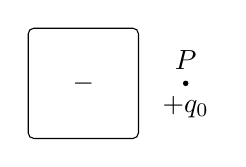
\begin{tikzpicture}
\draw[rounded corners=2pt] (0,0) rectangle (1.4,1.4);
\draw (0.7,0.7) node {$-$};
\fill (2,0.7) circle (1pt);
\draw (2,1) node {$P$};
\draw (2,0.4) node {$+q_0$};
\end{tikzpicture}
图7.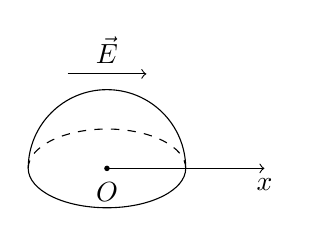
\begin{tikzpicture}
\draw (0,0) arc [start angle=0, end angle=180, x radius=1, y radius=1];
\draw[dashed] (0,0) arc [start angle=0, end angle=180, x radius=1, y radius=0.5];
\draw (0,0) arc [start angle=360, end angle=180, x radius=1, y radius=0.5];
\draw[->] (-1.5,1.2) -- (-0.5,1.2);
\draw (-1,1.5) node {$\vec E$};
\fill (-1,0) circle (1pt);
\draw (-1,-0.3) node {$O$};
\draw[->] (-1,0) -- (1,0);
\draw (1,-0.2) node {$x$};
\end{tikzpicture}
图8.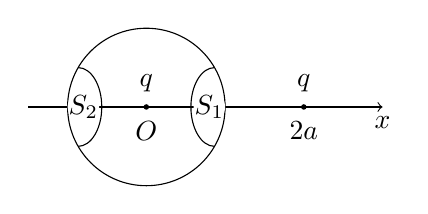
\begin{tikzpicture}
\draw (0,0) circle (1);
\fill (0,0) circle (1pt);
\draw (0,0.3) node {$q$};
\draw (0,-0.3) node {$O$};
\draw[->] (-1.5,0) -- (3,0);
\draw (3,-0.2) node {$x$};
\fill (2,0) circle (1pt);
\draw (2,0.3) node {$q$};
\draw (2,-0.3) node {$2a$};
\draw (30:1) arc [start angle=90, delta angle=180, y radius=0.5, x radius=0.3];
\fill[white] (0.8,0) circle (0.2);
\draw (0.8,0) node {$S_1$};
\draw (210:1) arc [start angle=270, delta angle=180, y radius=0.5, x radius=0.3];
\fill[white] (-0.8,0) circle (0.2);
\draw (-0.8,0) node {$S_2$};
\end{tikzpicture}

7. 一电场强度为$\vec E$的均匀电场,$\vec E$的方向沿$x$轴正方向,如图,则通过图中一半径为$R$的半球面的电场强度通量为\fbox{0}.

8. 有两个电荷都是$+q$的点电荷,相距为$2a$.今以左边的点电荷所在处为球心,以$a$为半径作一球形高斯面.在球面上取两块相等的小面积$S_1$和$S_2$,其位置如图所示.设通过$S_1$和$S_2$的电场强度通量分别为$\varPhi_1$和$\varPhi_2$,通过整个球面的电场强度通量为$\varPhi_S$,则\fbox{$\varPhi_1<\varPhi_2, \varPhi_S=q/\varepsilon_0$}.

\subsubsection*{二. 填空题}

\subsubsection*{三. 计算题}

\section*{稳恒磁场}

\subsubsection*{一. 选择题}

1. 在磁感强度为$\vec B$的均匀磁场中作一半径为$r$的半球面$S$,$S$边线所在平面的发现方向单位矢量$\vec n$与$\vec B$的夹角为$\alpha$,则通过半球面$S$的磁通量为\fbox{$-\pi r^2B\cos\alpha$}.(取弯曲面向外为正)

2. 边长为$a$的正方形的四个角上固定有四个电荷均为$q$的点电荷.此正方形以角速度$\omega$绕$AC$轴旋转时,在中心$O$点产生的磁感强度大小为$B_1$;此正方形以同样的角速度$\omega$绕过$O$点垂直于正方形平面的轴旋转时,在$O$点产生的磁感强度的大小为$B_2$,则\fbox{$B_1=\frac{1}{2}B_2$}.

3. 通有电流$I$的无限长直导线有如图三种形状(直线、“L”型、下半圆),则$P,Q,O$各点磁感强度大小关系为\fbox{$B_O>B_Q>B_P$}.

4. 载流的圆形线圈(半径$a_2$)与正方形线圈(边长$a_2$)通有相同电流$I$.若两个线圈的中心$O_1,O_2$处的磁感强度大小相同,则半径$a_1$与边长$a_2$的比$a_1:a_2$为\fbox{$\sqrt2\pi:8$}.

5. 无限长直导线在$P$弯成半径为$R$的圆,当通以电流$I$时,则在圆心$O$的磁感强度大小等于\fbox{$\frac{\mu_0I}{2R}(1-\frac{1}{\pi})$}.

6. 一个电流元$I\d\vec l$位于直角坐标系原点,电流沿$z$轴方向,点$P(x,y,z)$的磁感强度沿$x$轴的分量是\fbox{$-(\mu_0/4\pi)Iy\d l/(x^2+y^2+z^2)^{3/2}$}.

9. 电流由长直导线1沿半径方向经$a$点流入一由电阻均匀的导线构成的圆环,再由$b$点沿半径方向从圆环流出,经长直导线2返回电源.已知直导线上电流强度为$I$,$\angle aOb=30\degree$.若长直导线1,2和圆环中的电流在圆心$O$点产生的磁感强度分别用$\vec B_1,\vec B_2,\vec B_3$表示,则圆心$O$点的磁感强度大小\fbox{$B=0$,因为$B_1=B_2=B_3=0$}.

14. 有一无限长通电流的扁平铜片,宽度为$a$,厚度不计,电流$I$在铜片上均匀分布,在铜片外与铜片共面,离铜片右边缘为$b$处的$P$点的磁感强度$\vec B$的大小为\fbox{$\frac{\mu_0I}{2\pi a}\ln\frac{a+b}{b}$}.

15. 若空间存在两根无限长直载流导线,空间的磁场分布就不具有简单的对称性,则该磁场分布\ul{可以用安培环路定理和磁感强度的叠加原理求出}.

16. 如图,流出纸面的电流为$2I$,流进纸面的电流为$I$,则正确的是\fbox{$\oint_{L_4}\vec B\cdot\d\vec l=-\mu_0I$}.

17. 在图(a)和(b)中各有一半径相同的圆形回路$L_1,L_2$,圆周内有电流$I_1,I_2$,其分布相同,且均在真空中,但在(b)图中$L_2$回路外有电流$L_3$,$P_1,P_2$位两圆形回路上的对应点,则\fbox{$\oint_{L_1}\vec B\cdot\d\vec l=\oint_{L_2}\vec B\cdot\d\vec l$, $B_{P_1}\neq B_{P_2}$}.

20. 如图所示,在磁感强度为$\vec B$的均匀磁场中,有一圆形载流导线,$a,b,c$是其上三个长度相等的电流元,则它们所受安培力大小关系为\fbox{$F_b>F_c>F_a$}.

21. 如图,无限长直载流导线与正三角形载流线圈在同一平面内,若长直导线固定不动,则载流三角形线圈将\fbox{向着长直导线平移}.

22. 长直电流$I_2$与圆形电流$I_1$共面,并与其一直径相重合,如图(但两者间绝缘),设长直电流不懂,则圆形电流将\fbox{向右运动}.

25. 如图,匀强磁场中有一矩形铜电线圈,它的平面与磁场平行,在磁场作用下,线圈发生转动,其方向是\fbox{$ab$边转入纸内,$cd$边转出纸外}.

26. 把通电的直导线放在蹄形磁铁磁极的上方,如图所示.导线可以自由活动,且不计重力.当导线内通以如图所示的电流时,导线将\fbox{顺时针方向转动,然后下降}(从上往下看).

\subsubsection*{二. 填空题}

38. 真空中稳恒电流$I$流过两个半径分别为$R_1,R_2$的同心半圆型导线,两半圆导线间由沿直径的指导线连接,电流沿直导线流入.
    (1) 如果两个半圆共面(图1),圆心$O$点的磁感强度$\vec B_0$的大小为\fbox{$\frac{\mu_0I}{4}(\frac{1}{R_2}-\frac{1}{R_1})$},方向\fbox{垂直纸面向外};
    (2) 如果两个半圆正交(图2),则圆心$O$点的磁感强度$\vec B_0$的大小为\fbox{$\frac{\mu_0I}{4}\sqrt{\frac{1}{R_1^2}+\frac{1}{R_2^2}}$},$\vec B_0$的方向与$y$轴的夹角为\fbox{$\frac{2}{\pi}+\arctan\frac{R_2}{R_1}$}.

39. 一弯曲的载流导线在同一平面内,形状如图($O$点是半径为$R_1$和$R_2$的两个半圆弧的共同圆心,电流自无穷远来到无穷远去),则$O$点磁感强度的大小是\fbox{$B_0=\frac{\mu_0I}{4R_1}+\frac{\mu_0I}{4R_2}-\frac{\mu_0I}{4\pi R_2}$}.

49. 如图,在无限长直载流导线的右侧有面积为$S_1$和$S_2$的两个矩形回路.两回路与长直载流导线共面,且矩形回路的一边与长直载流导线平行.则通过面积为$S_1$的矩形回路的磁通量与通过面积为$S_2$的矩形回路的磁通量之比为\fbox{$1:1$}.

50. 有一同轴电缆,其尺寸如图所示,它的内外两导体中的电流均为$I$,且在横截面上均匀分布,点两者电流的流向正相反,则
    (1) 在$r<R_1$处磁感强度大小为\fbox{$\mu_0rI/(2\pi R_1^2)$};
    (2) 在$r>R_2$处磁感强度大小为\fbox{$0$}.

51. 两根长直导线通有电流$I$,图示有三种环路;在每种情况下,$\oint_L\vec B\cdot\d\vec l$等于:
    \fbox{$\mu_0I$}(对环路$a$),
    \fbox{$0$}(对环路$b$),
    \fbox{$2\mu_0I$}(对环路$c$).

65. 如图所示,在真空中有一半径为$a$的$3/4$圆弧形导线,其中通以稳恒电流$I$,导线置于均匀外磁场$\vec B$中,且$\vec B$与导线所在平面垂直.则该载流导线${bc}$所受磁力大小为\fbox{$\sqrt2aIB$}.

66. 如图所示,在真空中有一半圆形闭合线圈,半径为$a$,流过稳恒电流$I$,则圆心$O$处的电流元$I\d\vec l$所受的安培力$\d\vec F$的大小为\fbox{$\mu_0I^2\d l/4a$},方向\fbox{垂直电流元背向半圆弧(即向左)}.

\subsubsection*{三. 计算题}

69. 有一条载有电流$I$的导线弯成如图示$abcda$形状.其中$ab,cd$是直线段,其余为圆弧.两段圆弧的长度和半径分别为$I_1,R_1$和$I_2,R_2$,且两段圆弧共面共心.求圆心$O$处的磁感强度$\vec B$的大小.
\SL{两段圆弧在$O$处产生的磁感强度为$B_1=\frac{\mu_0Il_1}{4\pi R_1^2}$,$B_2=\frac{\mu_0Il_2}{4\pi R_2^2}$.\\
两段直导线在$O$处产生的磁感强度为$B_3=B_4=\frac{\mu_0I}{4\pi R_1\cos\frac{l_1}{2R_1}}(-\sin\frac{l_1}{2R_1}+\sin\frac{l_2}{2R_2})$.\\
取向里为正$B=B_1+B_3+B_4-B_2=\frac{\mu_0I}{2\pi R_1\cos\frac{l_1}{2R_1}}(-\sin\frac{l_1}{2R_1}+\sin\frac{l_2}{2R_2})+\frac{\mu_0I}{4\pi}(\frac{l_1}{R_1^2}-\frac{l_2}{R_2^2})$.
方向垂直版面向里.
}
71. 已知半径为$R$的载流圆线圈与边长为$a$的载流正方形线圈的磁矩之比为$2:1$,且载流圆线圈在中心$O$处产生的磁感应强度为$B_0$,求在正方形线圈中心$O'$处磁感强度的大小.
\SL{设圆线圈磁矩为$p_{m_1}$,方线圈磁矩为$p_{m_2}$,则$p_{m_1}=I_1\pi R^2$, $p_{m_2}=I_1a^2$,\\
所以$I_2=\pi R^2I_1/(2a^2)$.
正方形一边在其中心处产生的磁感强度\pp
$B_1=\frac{\mu_0I_2}{4\pi(a/2)}(\cos\frac{\pi}{4}-\frac{3\pi}{4})=\frac{\sqrt2\mu_0I_2}{2\pi a}$,
【答案缺失】
}
73. 将通有电流$I$的导线在同一平面内弯成如图所示形状,求$D$点的磁感强度$\vec B$的大小.
\SL{【答案缺失】
}
78. 用两根彼此平行的半无限长直导线$L_1,L_2$把半径为$R$的均匀导体圆环联到电源上,如图所示.已知直导线中的电流为$I$,求圆环中心$O$点的磁感强度.
\SL{【答案缺失】
$\vec B_3+\vec B_4=0$.\\
故$O$点的磁感强度$|\vec B_0|=|\vec B_1+\vec B_2+\vec B_3+\vec B_4|=\frac{\mu_0I}{4\pi R}$,方向垂直图面向外.
}
79. 如图所示,一无限长载流平板宽度为$a$,线电流密度为$\delta$(即沿$x$方向单位长度上的电流),求与平板共面且距平板一边为$b$的任意点$P$的磁感强度.
\SL{利用无限长载流直导线的公式求解.\\
取离$P$点为$x$宽度为$\d x$的无限长载流细条,它的电流$\d i=\delta\d x$,\\
这载流长条在$P$点产生的磁感强度
$\d B=\frac{\mu_0\d i}{2\pi x}=\frac{\mu_0\delta\d x}{2\pi x}$,
方向垂直纸面向里.\\
所有载流长条在$P$点产生的磁感强度方向都相同,所以载流平板在$P$点产生的磁感强度\pp
$B=\int\d B=\frac{\mu_0\delta}{2\pi x}\int_b^{a+b}\frac{\d x}{x}=\frac{\mu_0\delta}{2\pi x}\ln\frac{a+b}{b}$,
方向垂直纸面向里.
}
80. 在一无限长的半圆筒形的金属箔片中,沿轴向流有电流,在垂直电流方向单位长度的电流为$i=k\sin\theta$,其中$k$为常量,$\theta$如图所示.求半圆筒轴线上的磁感强度.
\SL{设轴线上任意点的磁感强度为$B$,半圆筒半径为$R$.\\
先将半圆筒面分成许多平行轴线宽度为$\d l$的无限长直导线,其中流过的电流为\pp
$\d I=i\d l=k\sin\theta\cdot\d l=k\sin\theta R\d\theta$,\\
它在轴线上产生的元磁感强度为
$\d B=\frac{\mu_0\d I}{2\pi R}$,方向如图.\\
由对称性可知:
$\d\vec B$在$z$轴向的分量为0,在$y$轴的分量叠加中互相抵消,\\
只需要考虑$\d\vec B$在$x$轴的分量
$\d B_x=\d B\sin\theta=\frac{\mu_0\d I}{2\pi R}\sin\theta=\frac{\mu_0k\sin^2\theta}{2\pi}\d\theta$,\\
积分
$B=\int\d B_x=\int_0^\pi\frac{\mu_0k\sin^2\theta}{2\pi}\d\theta=\frac{\mu_0k}{2\pi}\int_0^\pi\frac{1-\cos2\theta}{2}\d\theta=\frac{\mu_0k}{4}$.
}
81. 如图所示,载有电流$I_1$和$I_2$的长直导线$ab$和$cd$相互平行,相距为$3r$,今有载有电流$I_3$的导线$MN=r$,水平放置,且其两端$MN$分别与$I_1,I_2$的距离都是$r$, $ab,cd$和$MN$共面,求导线$MN$所受的磁力大小和方向.
\SL{载流导线$MN$上任一点处的磁感强度大小为
$B=\frac{\mu_0I_1}{2\pi(r+x)}-\frac{\mu_0I_2}{2\pi(2r-x)}$.\\
$MN$上电流元$I_3\d x$所受磁力
$\d F=I_3B\d x=I_3[\frac{\mu_0I_1}{2\pi(r+x)}-\frac{\mu_0I_2}{2\pi(2r-x)}]\d x$,\pp
$F\,= I_3\int_0^r[\frac{\mu_0I_1}{2\pi(r+x)}-\frac{\mu_0I_2}{2\pi(2r-x)}]\d x
   = \frac{\mu_0I_1}{2\pi}[\int_0^r\frac{I_1}{r+x}\d x-\int_0^r\frac{I_2}{2r-x}\d x]
$\\  
$  = \frac{\mu_0I_1}{2\pi}[I_1\ln\frac{2r}{r}+I_2\ln\frac{r}{2r}]
   = \frac{\mu_0I_1}{2\pi}[I_1\ln2-I_2\ln2]
   = \frac{\mu_0I_1}{2\pi}(I_1-I_2)\ln2$.\\
若$I_2>I_1$,则$\vec F$的方向向下;
若$I_2<I_1$,则$\vec F$的方向向上.
}

\section*{电磁感应}

\subsubsection*{一. 选择题}
\subsubsection*{二. 填空题}
\subsubsection*{三. 计算题}

% \end{multicols}

\end{document}
